\documentclass{sig-alternate}

\title{CS 472 --- Project 3}
\subtitle {GAs \& DEs --- A Land of Lisp Approach}

\numberofauthors{1}

\author{
\alignauthor
Steven White \\
  \email{swhite24@mix.wvu.edu}\\
  8258
}

\begin{document}
\date{22 March 2012}
\pagenumbering{arabic}

\maketitle
\section{abstract}
Test drive abstract. More to come.  Need to list all subsequent
sections along with a brief summary.

\section{Introduction}
The purpose of this project is to objectively compare two subsets of evolutionary algorithms, differential evolution (DE) and genetic algorithms (GA), using the model of evolving rats found in Conrad Barski's \emph{Land of Lisp}.  The two sets of algorithms will be tested for success in several criteria --- run-time, diversity of population, scoring, and time taken to achieve a stable population.

The algorithms will be tested with both a single-objective and multiple-objective version of the evolving rats problem.  The simplest and most obvious objectives to use in the context of this problem are the amount of energy a candidate has in comparison to the maximum potential energy and the number of children a candidate has produced relative to its age.  Due to the nature of these objectives and the model itself, a slight diversion was made from the traditional versions of DEs and GAs which immediately compare the scores of candidates with parents.  Instead, we will allow the candidates free roam for a period of generations, in order to be able to accurately assess their success.  Once a candidate is of correct of age, it will be compared with its parent.  Each objective will be scored independently and will be unweighted.  If a candidate dominates the parent, the parent will be removed from future generations.  Conversely, if a candidate is dominated by the parent, the candidate will be removed.  If neither the parent nor the candidate dominate the other, both will remain for future generations.

In addition to comparing one algorithm set with the other, each set will be compared to itself by changing their corresponding choice options, such as scaling factor when mutating, cross-over frequency, and population size.  Changing these options will affect each of the previously listed comparative criteria and may also arrive at a better solution.

\section{Model}

\subsection{World Description}
The model to be used for both differential evolution and genetic algorithms will be the rat evolution model of \emph{Land of Lisp}.  This model evolves a randomly generated initial population of a single rat.  The landscape of the ``world'' is thirty units tall by one hundred units wide.  The rats are herbivores, and the landscape is populated with two additional plants for each generation.  Rats have a set amount of energy, and must find plants to regain lost energy in order to remain alive.  Should a rat's energy reach zero, the rat will die and be removed from further generations.  A central ``oasis'' is present in the landscape.  Of the two plants placed in the landscape for each generation, one will be placed randomly inside the oasis, and the other placed randomly somewhere outside the oasis. 

Each generation of this model involves a specific life-cycle of the rats.  The first thing rats do is turn.  The direction of the turn is determined by the rat's genes.  Each rat has a set of genes corresponding to how likely they are to turn a certain direction.  A visual depiction of this these genes and their corresponding directions is shown in Figure 1.  \begin{figure}
\centering
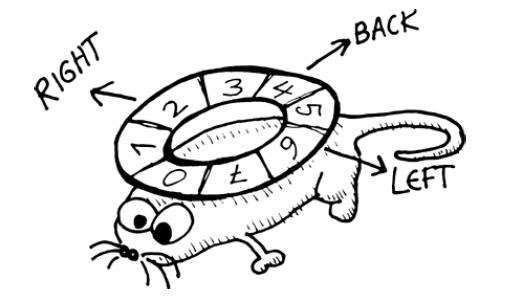
\includegraphics[width=0.4\textwidth]{rat_wheel.PNG}
\caption{Gene ``wheel'' depicting directions of rat travel.}
\end{figure}
For example, a rat with higher values in the lower-indexed positions of the gene will make less dramatic turns.  

Once turned, the next step in a rat's life-cycle is to move in the specified direction.  Due to the centrally located oasis, two distinct types of genes are expected to evolve.  The first will have higher valued genes with lower indexes, causing them to run at a more constant direction and often returning to the oasis.  The second will have higher valued genes with higher indexes, causing them to wander around a fairly consistent area, i.e. the oasis.  

The final step in the life-cycle of a rat is to produce offspring.  In order for a rat to be eligible to reproduce, a minimum energy requirement must be met.  Should that requirement be met, the total energy of the parent is split equally between itself and the offspring.  The genes of the offpring are uniquely generated by each algorithm, though a basic premise remains that offpsring are similar, but typically not identical, to their parent.

\subsection{Modifications for our Purposes}
Unlike the original version, the model used for all experiments described later had an initial population of four rats.  The primary reason for this difference is that differential evolution requires the parent and three other randomly generated rats for the parent to produce offspring.  An initial population of just a single rat would prevent any diversity in the population of rats, merely a horde of clones.  The same setup was used for genetic algorithsm simply for consistency.

Staying true to traditional evolutionary algorithms, offspring will compete with parents for a position in future generations.  Once a child is of sufficient age, it will be scored and compared to its parent, with the victor living on.  This presents two distinct possibilities of rats being terminated.  This is different from the original model in which rats only died if their energy reached zero.  

\subsection{Decision Space}
The decision space of this model consists entirely of the genes of each rat.  No other controllable factor has so large an effect of the success of an individual.  

\subsection{Objective Space}


\section{Algorithms}
Compare and constrast DE with GA.  Some pseudo-code.

\subsection{Genetic Algorithms}
GA specific alg info here.

\subsection{Differential Evolution}
DE specific alg info here. Only using DEMO/parent at this point.

\subsection{Comparison}
Compare \& contrast GA with DE.

\section{Expectations}
List of research questions (RQ1, RQ2, etc) and/or hypotheses
(H1, H2, etc).  Must include two-population hypothesis.

\section{Results}
Performance, effectiveness, better on one or multiple
objectives.  Graphs, etc.

\section{Validity}
Comment on limitations of study.

\section{Conclusion}
Return to section \emph{Expectations} and address whether the results
match what was expected.

\section{Further Work}
Discuss paths not taken.  What would be next step?

\section{References}
Self-explanatory.

\section{Listings}
All source code and example output.  Divide code into three files
--- de.lisp, ga.lisp, and gade.lisp.

\end{document}
